\documentclass[a4paper]{ctexart}
\usepackage{xltxtra}
\usepackage{minted}
\usepackage{tabularx}

\title{作业2: Shell脚本与信号}
\author{李志阳 \\ 混合班 3190105480}
\begin{document}
\maketitle

\section{Linux的信号}

我们常常使用Ctrl+C来终止程序的运行, 那么这个Ctrl+C是什么呢? 它工作的原理又是什么呢? 其实,  在Linux中, 这样的东西被称为\textbf{信号}(Signal).

信号是一种进程间通信的方式, 既然是通信, 也就是说会有一个程序负责发送信号,  另一个程序负责接收。这个发送的程序可以是任意运行中的程序, 包括终端。当按下Ctrl+C时,  就是由终端向我们的程序发送一个SIGINT信号, 在没有特定接收信号的动作的情况下,  程序接收到信号之后都会有默认的行为, 比如接收到Ctrl+C时,  默认为终止程序。类似的信号还包括SIGKILL(用于杀死进程), SIGCHLD(用于标志子进程的结束)等等.

下面是一张常见信号及其默认行为的列表:
\begin{table}[ht]
% \caption{常见信号及默认动作}\label{}
\small
\begin{tabularx}{\textwidth}{|p{2cm}|p{1cm}|p{2cm}|X|}
% \normalsize
      \hline
      \textbf{信号名称} & \textbf{信号数值} & \textbf{默认动作} & \textbf{描述}\\
      \hline
      SIGHUP & 1 & 终止进程 & 终端连接结束时发出。终端连接断开,会向当前终端连接会话关联的所有前台和后台进程组发送SIGHUP信号,用于终止进程。\\
      \hline
      SIGINT & 2 & 终止进程 & 程序终止(interrupt)信号, 通常是Ctrl+C发出。\\
      \hline
      SIGQUIT & 3 & 终止进程 & 和SIGINT类似,通常是Ctrl+/发出。进程在收到SIGQUIT信号退出时会产生core文件, 在这个意义上类似于一个程序错误信号。\\
      \hline
\end{tabularx}
\end{table}
\begin{table}[ht]
\small
\begin{tabularx}{\textwidth}{|p{2cm}|p{1cm}|p{2cm}|X|}
      \hline 
      SIGFPE & 8 & 终止进程,建立CORE文件 & 在发生致命的算术运算错误(Floating-Point Exception)时发出,不仅包括浮点运算错误, 还包括溢出及除数为0等其它所有的算术错误。\\
      \hline 
      SIGKILL & 9 & 终止进程 & 用来立即结束程序的运行。本信号不能被阻塞, 处理和忽略。\\
      \hline 
      SIGSEGV & 11 & 终止进程,建立CORE文件 & 段错误(Segmentation Fault)信号。进程试图访问非法内存地址,如往没有写权限的内存地址写数据时会触发段错误。\\
      \hline
      SIGALRM & 14 & 终止进程 & 时钟定时信号, 计时器到时会发出该信号。alarm()函数使用该信号。\\
      \hline
      SIGTERM & 15 & 终止进程 & 程序结束(Terminate)信号, 与SIGKILL不同的是该信号可以被阻塞和处理。通常用来要求程序自己正常退出。Shell命令kill缺省产生这个信号。\\
      \hline
      SIGCHLD & 17 & 忽略信号 & 子进程结束时, 父进程会收到这个信号\\
      \hline
\end{tabularx}
\end{table}
\\\\

发送信号的方式也有很多, 比如上面提到的使用Ctrl+C向运行中的进程发送SIGINT信号. 常见的kill命令也可以用于发送信号(In fact, kill命令本来就是用来发信号的, 而不是终止进程). 其用法为:

\begin{minted}{shell}
kill [-<信息名称或编号>][程序]
\end{minted}

其中, 程序可以是进程号, 也可以是作业号. \verb|-s|后面的参数用来表示要发送的信号, 使用时用上表中的信号名称去掉SIG表示, 也可以由信号数值表示. 比如:

\begin{minted}{shell}
kill -KILL 123456
\end{minted}

表示向PID为123456的进程发送SIGKILL信号, 同样的, 这条命令也可以写为:

\begin{minted}{shell}
kill -9 123456
\end{minted}

\section{在shell中处理信号}
\subsection{trap命令}
在shell中处理信号, 使用\verb|trap|命令. trap命令有如下两种用法:
\begin{itemize}
    \item 
\begin{minted}{shell}
   trap 'commands' signal-list
或 trap "commands" signal-list
\end{minted}

这种形式用于改变程序接收到信号的行为, 接收到\verb!signal-list!中的信号(同样用上表中的名字去掉SIG或序号表示)时, 将执行的默认动作改为\verb|commands|中的命令, 如:
\begin{minted}{shell}
trap "echo 'trapped';" INT
\end{minted}

表示接收到SIGINT信号, 不再终止运行, 而是输出trapped.
当commands为空时, 不执行任何命令.
    \item \begin{minted}{shell}
   trap signal-list
\end{minted}
这种情况表示恢复该信号的默认操作.
\end{itemize}
\subsection{try-out}

书上提供如下例子(P60):
\begin{minted}{shell}
trap 'rm -f /tmp/my_tmp_file_$$' INT
echo creating file /tmp/my_tmp_file_$$
date > /tmp/my_tmp_file_$$
echo "press interrupt (CTRL-C) to interrupt ...."
while [ -f /tmp/my_tmp_file_$$ ]; do
    echo File exists
    sleep 1
done
echo The file no longer exists
trap INT
echo creating file /tmp/my_tmp_file_$$
date > /tmp/my_tmp_file_$$
echo "press interrupt (control-C) to interrupt ...."
while [ -f /tmp/my_tmp_file_$$ ]; do
    echo File exists
    sleep 1
done
echo we never get here
exit 0
\end{minted}

这段代码中, 先使用当前PID确定一个文件名, 将日期写入这个文件中, 然后不断循环输出File exists. 

当按下Ctrl+C时, 程序接收到信号SIGINT. 因为在第一行使用\verb|trap|将SIGINT的动作变更为了删除这一文件, 因此这时程序将执行删除而非退出. 这时循环条件已不满足(因为循环条件是文件存在时继续), 脚本退出循环.

继续执行\verb|echo The file no longer exists|. 而后将SIGINT的处理恢复默认并重新创建文件, 然后进入新的循环,  不断输出File exists. 在这时按下Ctrl+C, 则会执行默认动作退出程序, 否则会一直执行这一循环. 因此后面的echo是不可到达的.

这里是一张执行截图:
\begin{figure}[htbp]
    \centering
    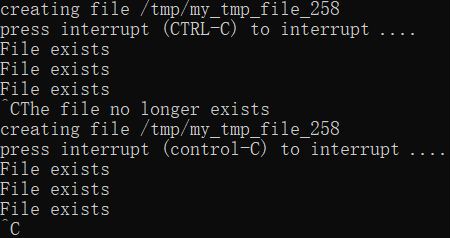
\includegraphics[scale=0.8]{HW2_截图.png}
    \caption{运行结果1}
\end{figure} 

在\^C处按下了Ctrl+C, 可以看到第一次按下时并没有终止执行. 第二次按下时才退出.
运行结束时查看/tmp, 发现文件仍然存在:
\begin{figure}[htbp]
    \centering
    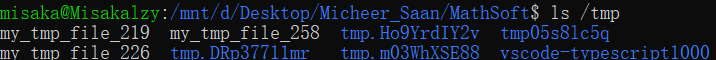
\includegraphics[scale=0.8]{HW2_截图1.png}
    \caption{查看/tmp}
\end{figure} 

于是, 产生了一个有趣的想法, 在按下第一次Ctrl+C后手动删掉文件会如何? 按理说应该会循环条件不满足退出, 下面进行验证:
\begin{figure}[htbp]
    \centering
    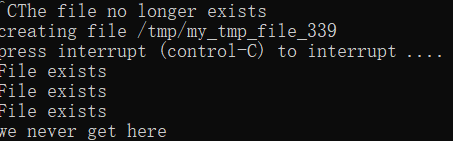
\includegraphics[scale=0.8]{HW2_截图2.png}
    \caption{运行结果2}
\end{figure} 

确实输出了We never get here.

更进一步, 我们可以尝试trap命令嵌套使用, 比如:
\begin{minted}{shell}
trap 'echo "hh" && trap "echo hi && trap INT" INT' INT
echo creating file /tmp/my_tmp_file_$$
date > /tmp/my_tmp_file_$$
echo "press interrupt (CTRL-C) to interrupt ...."
while [ -f /tmp/my_tmp_file_$$ ]; do
    echo File exists
    sleep 1
done
echo Strange
exit 0
\end{minted}

第一次trap时, 将INT的操作改为了输出hh并执行第二个trap, 第二次trap时, 将INT的操作改为输出hi并恢复默认操作. 因此我们第一次Ctrl+C时, 输出hh, 第二次输出hi, 第三次退出. 验证:
\begin{figure}[htbp]
    \centering
    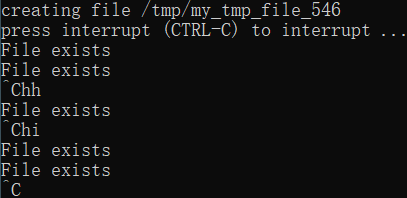
\includegraphics[scale=0.8]{HW2_截图3.png}
    \caption{运行结果3}
\end{figure} 






\bibliographystyle{plain}
\bibliography{crazyfish.bib}

\end{document}